\makesection{Conclusion}

\begin{frame}{Conclusion}

    \begin{itemize}
        \item Achievements:
        \begin{multicols}{4}
            \begin{tcolorbox}[colback=boxcolor, colframe=boxcolor, width=0.235\textwidth, height=4.5cm, rounded corners]
                \centering
                Modular and maintainable architecture and optimized codebase.
            \end{tcolorbox}
            
            \begin{tcolorbox}[colback=boxcolor, colframe=boxcolor, width=0.235\textwidth, height=4.5cm, rounded corners]
                \centering
                Design of a customizable physics engine which supports convex polygons.
            \end{tcolorbox}
            
            \begin{tcolorbox}[colback=boxcolor, colframe=boxcolor, width=0.235\textwidth, height=4.5cm, rounded corners]
                \centering
                Framework (based on OOP) that can be readily extended.
            \end{tcolorbox}
            
            \begin{tcolorbox}[colback=boxcolor, colframe=boxcolor, width=0.235\textwidth, height=4.5cm, rounded corners]
                \centering
                Enhanced user experience with new features (terrain, items, graphics..)
            \end{tcolorbox}
        \end{multicols}
        \item Tradeoff: OOP architecture is less performant than flecs.
    \end{itemize}
\end{frame}

\begin{frame}{Future Work}
    \begin{itemize}
        \item Multiplayer modes and leaderboard integration.
        \item New game items and biomes.
        \item Difficulty settings, coin shop to buy upgrades
        \item Further enhancements to the physics engine:
        \begin{itemize}
            \item Improved performance with parallel batch processing and spatial data structures.
            \item Friction and air resistance.
            \item Reduction of jitter.
        \end{itemize}
    \end{itemize}
    \centering
    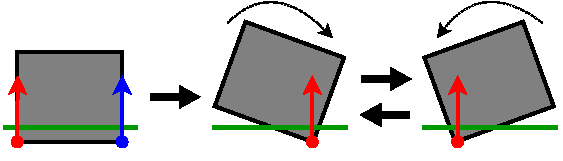
\includegraphics[width = .5\textwidth]{../figures/physics/jitter.pdf}
\end{frame}